
% Default to the notebook output style

    


% Inherit from the specified cell style.




    
\documentclass[11pt]{article}

    
    
    \usepackage[T1]{fontenc}
    % Nicer default font (+ math font) than Computer Modern for most use cases
    \usepackage{mathpazo}

    % Basic figure setup, for now with no caption control since it's done
    % automatically by Pandoc (which extracts ![](path) syntax from Markdown).
    \usepackage{graphicx}
    % We will generate all images so they have a width \maxwidth. This means
    % that they will get their normal width if they fit onto the page, but
    % are scaled down if they would overflow the margins.
    \makeatletter
    \def\maxwidth{\ifdim\Gin@nat@width>\linewidth\linewidth
    \else\Gin@nat@width\fi}
    \makeatother
    \let\Oldincludegraphics\includegraphics
    % Set max figure width to be 80% of text width, for now hardcoded.
    \renewcommand{\includegraphics}[1]{\Oldincludegraphics[width=.8\maxwidth]{#1}}
    % Ensure that by default, figures have no caption (until we provide a
    % proper Figure object with a Caption API and a way to capture that
    % in the conversion process - todo).
    \usepackage{caption}
    \DeclareCaptionLabelFormat{nolabel}{}
    \captionsetup{labelformat=nolabel}

    \usepackage{adjustbox} % Used to constrain images to a maximum size 
    \usepackage{xcolor} % Allow colors to be defined
    \usepackage{enumerate} % Needed for markdown enumerations to work
    \usepackage{geometry} % Used to adjust the document margins
    \usepackage{amsmath} % Equations
    \usepackage{amssymb} % Equations
    \usepackage{textcomp} % defines textquotesingle
    % Hack from http://tex.stackexchange.com/a/47451/13684:
    \AtBeginDocument{%
        \def\PYZsq{\textquotesingle}% Upright quotes in Pygmentized code
    }
    \usepackage{upquote} % Upright quotes for verbatim code
    \usepackage{eurosym} % defines \euro
    \usepackage[mathletters]{ucs} % Extended unicode (utf-8) support
    \usepackage[utf8x]{inputenc} % Allow utf-8 characters in the tex document
    \usepackage{fancyvrb} % verbatim replacement that allows latex
    \usepackage{grffile} % extends the file name processing of package graphics 
                         % to support a larger range 
    % The hyperref package gives us a pdf with properly built
    % internal navigation ('pdf bookmarks' for the table of contents,
    % internal cross-reference links, web links for URLs, etc.)
    \usepackage{hyperref}
    \usepackage{longtable} % longtable support required by pandoc >1.10
    \usepackage{booktabs}  % table support for pandoc > 1.12.2
    \usepackage[inline]{enumitem} % IRkernel/repr support (it uses the enumerate* environment)
    \usepackage[normalem]{ulem} % ulem is needed to support strikethroughs (\sout)
                                % normalem makes italics be italics, not underlines
    

    
    
    % Colors for the hyperref package
    \definecolor{urlcolor}{rgb}{0,.145,.698}
    \definecolor{linkcolor}{rgb}{.71,0.21,0.01}
    \definecolor{citecolor}{rgb}{.12,.54,.11}

    % ANSI colors
    \definecolor{ansi-black}{HTML}{3E424D}
    \definecolor{ansi-black-intense}{HTML}{282C36}
    \definecolor{ansi-red}{HTML}{E75C58}
    \definecolor{ansi-red-intense}{HTML}{B22B31}
    \definecolor{ansi-green}{HTML}{00A250}
    \definecolor{ansi-green-intense}{HTML}{007427}
    \definecolor{ansi-yellow}{HTML}{DDB62B}
    \definecolor{ansi-yellow-intense}{HTML}{B27D12}
    \definecolor{ansi-blue}{HTML}{208FFB}
    \definecolor{ansi-blue-intense}{HTML}{0065CA}
    \definecolor{ansi-magenta}{HTML}{D160C4}
    \definecolor{ansi-magenta-intense}{HTML}{A03196}
    \definecolor{ansi-cyan}{HTML}{60C6C8}
    \definecolor{ansi-cyan-intense}{HTML}{258F8F}
    \definecolor{ansi-white}{HTML}{C5C1B4}
    \definecolor{ansi-white-intense}{HTML}{A1A6B2}

    % commands and environments needed by pandoc snippets
    % extracted from the output of `pandoc -s`
    \providecommand{\tightlist}{%
      \setlength{\itemsep}{0pt}\setlength{\parskip}{0pt}}
    \DefineVerbatimEnvironment{Highlighting}{Verbatim}{commandchars=\\\{\}}
    % Add ',fontsize=\small' for more characters per line
    \newenvironment{Shaded}{}{}
    \newcommand{\KeywordTok}[1]{\textcolor[rgb]{0.00,0.44,0.13}{\textbf{{#1}}}}
    \newcommand{\DataTypeTok}[1]{\textcolor[rgb]{0.56,0.13,0.00}{{#1}}}
    \newcommand{\DecValTok}[1]{\textcolor[rgb]{0.25,0.63,0.44}{{#1}}}
    \newcommand{\BaseNTok}[1]{\textcolor[rgb]{0.25,0.63,0.44}{{#1}}}
    \newcommand{\FloatTok}[1]{\textcolor[rgb]{0.25,0.63,0.44}{{#1}}}
    \newcommand{\CharTok}[1]{\textcolor[rgb]{0.25,0.44,0.63}{{#1}}}
    \newcommand{\StringTok}[1]{\textcolor[rgb]{0.25,0.44,0.63}{{#1}}}
    \newcommand{\CommentTok}[1]{\textcolor[rgb]{0.38,0.63,0.69}{\textit{{#1}}}}
    \newcommand{\OtherTok}[1]{\textcolor[rgb]{0.00,0.44,0.13}{{#1}}}
    \newcommand{\AlertTok}[1]{\textcolor[rgb]{1.00,0.00,0.00}{\textbf{{#1}}}}
    \newcommand{\FunctionTok}[1]{\textcolor[rgb]{0.02,0.16,0.49}{{#1}}}
    \newcommand{\RegionMarkerTok}[1]{{#1}}
    \newcommand{\ErrorTok}[1]{\textcolor[rgb]{1.00,0.00,0.00}{\textbf{{#1}}}}
    \newcommand{\NormalTok}[1]{{#1}}
    
    % Additional commands for more recent versions of Pandoc
    \newcommand{\ConstantTok}[1]{\textcolor[rgb]{0.53,0.00,0.00}{{#1}}}
    \newcommand{\SpecialCharTok}[1]{\textcolor[rgb]{0.25,0.44,0.63}{{#1}}}
    \newcommand{\VerbatimStringTok}[1]{\textcolor[rgb]{0.25,0.44,0.63}{{#1}}}
    \newcommand{\SpecialStringTok}[1]{\textcolor[rgb]{0.73,0.40,0.53}{{#1}}}
    \newcommand{\ImportTok}[1]{{#1}}
    \newcommand{\DocumentationTok}[1]{\textcolor[rgb]{0.73,0.13,0.13}{\textit{{#1}}}}
    \newcommand{\AnnotationTok}[1]{\textcolor[rgb]{0.38,0.63,0.69}{\textbf{\textit{{#1}}}}}
    \newcommand{\CommentVarTok}[1]{\textcolor[rgb]{0.38,0.63,0.69}{\textbf{\textit{{#1}}}}}
    \newcommand{\VariableTok}[1]{\textcolor[rgb]{0.10,0.09,0.49}{{#1}}}
    \newcommand{\ControlFlowTok}[1]{\textcolor[rgb]{0.00,0.44,0.13}{\textbf{{#1}}}}
    \newcommand{\OperatorTok}[1]{\textcolor[rgb]{0.40,0.40,0.40}{{#1}}}
    \newcommand{\BuiltInTok}[1]{{#1}}
    \newcommand{\ExtensionTok}[1]{{#1}}
    \newcommand{\PreprocessorTok}[1]{\textcolor[rgb]{0.74,0.48,0.00}{{#1}}}
    \newcommand{\AttributeTok}[1]{\textcolor[rgb]{0.49,0.56,0.16}{{#1}}}
    \newcommand{\InformationTok}[1]{\textcolor[rgb]{0.38,0.63,0.69}{\textbf{\textit{{#1}}}}}
    \newcommand{\WarningTok}[1]{\textcolor[rgb]{0.38,0.63,0.69}{\textbf{\textit{{#1}}}}}
    
    
    % Define a nice break command that doesn't care if a line doesn't already
    % exist.
    \def\br{\hspace*{\fill} \\* }
    % Math Jax compatability definitions
    \def\gt{>}
    \def\lt{<}
    % Document parameters
    \title{HW02}
    
    
    

    % Pygments definitions
    
\makeatletter
\def\PY@reset{\let\PY@it=\relax \let\PY@bf=\relax%
    \let\PY@ul=\relax \let\PY@tc=\relax%
    \let\PY@bc=\relax \let\PY@ff=\relax}
\def\PY@tok#1{\csname PY@tok@#1\endcsname}
\def\PY@toks#1+{\ifx\relax#1\empty\else%
    \PY@tok{#1}\expandafter\PY@toks\fi}
\def\PY@do#1{\PY@bc{\PY@tc{\PY@ul{%
    \PY@it{\PY@bf{\PY@ff{#1}}}}}}}
\def\PY#1#2{\PY@reset\PY@toks#1+\relax+\PY@do{#2}}

\expandafter\def\csname PY@tok@w\endcsname{\def\PY@tc##1{\textcolor[rgb]{0.73,0.73,0.73}{##1}}}
\expandafter\def\csname PY@tok@c\endcsname{\let\PY@it=\textit\def\PY@tc##1{\textcolor[rgb]{0.25,0.50,0.50}{##1}}}
\expandafter\def\csname PY@tok@cp\endcsname{\def\PY@tc##1{\textcolor[rgb]{0.74,0.48,0.00}{##1}}}
\expandafter\def\csname PY@tok@k\endcsname{\let\PY@bf=\textbf\def\PY@tc##1{\textcolor[rgb]{0.00,0.50,0.00}{##1}}}
\expandafter\def\csname PY@tok@kp\endcsname{\def\PY@tc##1{\textcolor[rgb]{0.00,0.50,0.00}{##1}}}
\expandafter\def\csname PY@tok@kt\endcsname{\def\PY@tc##1{\textcolor[rgb]{0.69,0.00,0.25}{##1}}}
\expandafter\def\csname PY@tok@o\endcsname{\def\PY@tc##1{\textcolor[rgb]{0.40,0.40,0.40}{##1}}}
\expandafter\def\csname PY@tok@ow\endcsname{\let\PY@bf=\textbf\def\PY@tc##1{\textcolor[rgb]{0.67,0.13,1.00}{##1}}}
\expandafter\def\csname PY@tok@nb\endcsname{\def\PY@tc##1{\textcolor[rgb]{0.00,0.50,0.00}{##1}}}
\expandafter\def\csname PY@tok@nf\endcsname{\def\PY@tc##1{\textcolor[rgb]{0.00,0.00,1.00}{##1}}}
\expandafter\def\csname PY@tok@nc\endcsname{\let\PY@bf=\textbf\def\PY@tc##1{\textcolor[rgb]{0.00,0.00,1.00}{##1}}}
\expandafter\def\csname PY@tok@nn\endcsname{\let\PY@bf=\textbf\def\PY@tc##1{\textcolor[rgb]{0.00,0.00,1.00}{##1}}}
\expandafter\def\csname PY@tok@ne\endcsname{\let\PY@bf=\textbf\def\PY@tc##1{\textcolor[rgb]{0.82,0.25,0.23}{##1}}}
\expandafter\def\csname PY@tok@nv\endcsname{\def\PY@tc##1{\textcolor[rgb]{0.10,0.09,0.49}{##1}}}
\expandafter\def\csname PY@tok@no\endcsname{\def\PY@tc##1{\textcolor[rgb]{0.53,0.00,0.00}{##1}}}
\expandafter\def\csname PY@tok@nl\endcsname{\def\PY@tc##1{\textcolor[rgb]{0.63,0.63,0.00}{##1}}}
\expandafter\def\csname PY@tok@ni\endcsname{\let\PY@bf=\textbf\def\PY@tc##1{\textcolor[rgb]{0.60,0.60,0.60}{##1}}}
\expandafter\def\csname PY@tok@na\endcsname{\def\PY@tc##1{\textcolor[rgb]{0.49,0.56,0.16}{##1}}}
\expandafter\def\csname PY@tok@nt\endcsname{\let\PY@bf=\textbf\def\PY@tc##1{\textcolor[rgb]{0.00,0.50,0.00}{##1}}}
\expandafter\def\csname PY@tok@nd\endcsname{\def\PY@tc##1{\textcolor[rgb]{0.67,0.13,1.00}{##1}}}
\expandafter\def\csname PY@tok@s\endcsname{\def\PY@tc##1{\textcolor[rgb]{0.73,0.13,0.13}{##1}}}
\expandafter\def\csname PY@tok@sd\endcsname{\let\PY@it=\textit\def\PY@tc##1{\textcolor[rgb]{0.73,0.13,0.13}{##1}}}
\expandafter\def\csname PY@tok@si\endcsname{\let\PY@bf=\textbf\def\PY@tc##1{\textcolor[rgb]{0.73,0.40,0.53}{##1}}}
\expandafter\def\csname PY@tok@se\endcsname{\let\PY@bf=\textbf\def\PY@tc##1{\textcolor[rgb]{0.73,0.40,0.13}{##1}}}
\expandafter\def\csname PY@tok@sr\endcsname{\def\PY@tc##1{\textcolor[rgb]{0.73,0.40,0.53}{##1}}}
\expandafter\def\csname PY@tok@ss\endcsname{\def\PY@tc##1{\textcolor[rgb]{0.10,0.09,0.49}{##1}}}
\expandafter\def\csname PY@tok@sx\endcsname{\def\PY@tc##1{\textcolor[rgb]{0.00,0.50,0.00}{##1}}}
\expandafter\def\csname PY@tok@m\endcsname{\def\PY@tc##1{\textcolor[rgb]{0.40,0.40,0.40}{##1}}}
\expandafter\def\csname PY@tok@gh\endcsname{\let\PY@bf=\textbf\def\PY@tc##1{\textcolor[rgb]{0.00,0.00,0.50}{##1}}}
\expandafter\def\csname PY@tok@gu\endcsname{\let\PY@bf=\textbf\def\PY@tc##1{\textcolor[rgb]{0.50,0.00,0.50}{##1}}}
\expandafter\def\csname PY@tok@gd\endcsname{\def\PY@tc##1{\textcolor[rgb]{0.63,0.00,0.00}{##1}}}
\expandafter\def\csname PY@tok@gi\endcsname{\def\PY@tc##1{\textcolor[rgb]{0.00,0.63,0.00}{##1}}}
\expandafter\def\csname PY@tok@gr\endcsname{\def\PY@tc##1{\textcolor[rgb]{1.00,0.00,0.00}{##1}}}
\expandafter\def\csname PY@tok@ge\endcsname{\let\PY@it=\textit}
\expandafter\def\csname PY@tok@gs\endcsname{\let\PY@bf=\textbf}
\expandafter\def\csname PY@tok@gp\endcsname{\let\PY@bf=\textbf\def\PY@tc##1{\textcolor[rgb]{0.00,0.00,0.50}{##1}}}
\expandafter\def\csname PY@tok@go\endcsname{\def\PY@tc##1{\textcolor[rgb]{0.53,0.53,0.53}{##1}}}
\expandafter\def\csname PY@tok@gt\endcsname{\def\PY@tc##1{\textcolor[rgb]{0.00,0.27,0.87}{##1}}}
\expandafter\def\csname PY@tok@err\endcsname{\def\PY@bc##1{\setlength{\fboxsep}{0pt}\fcolorbox[rgb]{1.00,0.00,0.00}{1,1,1}{\strut ##1}}}
\expandafter\def\csname PY@tok@kc\endcsname{\let\PY@bf=\textbf\def\PY@tc##1{\textcolor[rgb]{0.00,0.50,0.00}{##1}}}
\expandafter\def\csname PY@tok@kd\endcsname{\let\PY@bf=\textbf\def\PY@tc##1{\textcolor[rgb]{0.00,0.50,0.00}{##1}}}
\expandafter\def\csname PY@tok@kn\endcsname{\let\PY@bf=\textbf\def\PY@tc##1{\textcolor[rgb]{0.00,0.50,0.00}{##1}}}
\expandafter\def\csname PY@tok@kr\endcsname{\let\PY@bf=\textbf\def\PY@tc##1{\textcolor[rgb]{0.00,0.50,0.00}{##1}}}
\expandafter\def\csname PY@tok@bp\endcsname{\def\PY@tc##1{\textcolor[rgb]{0.00,0.50,0.00}{##1}}}
\expandafter\def\csname PY@tok@fm\endcsname{\def\PY@tc##1{\textcolor[rgb]{0.00,0.00,1.00}{##1}}}
\expandafter\def\csname PY@tok@vc\endcsname{\def\PY@tc##1{\textcolor[rgb]{0.10,0.09,0.49}{##1}}}
\expandafter\def\csname PY@tok@vg\endcsname{\def\PY@tc##1{\textcolor[rgb]{0.10,0.09,0.49}{##1}}}
\expandafter\def\csname PY@tok@vi\endcsname{\def\PY@tc##1{\textcolor[rgb]{0.10,0.09,0.49}{##1}}}
\expandafter\def\csname PY@tok@vm\endcsname{\def\PY@tc##1{\textcolor[rgb]{0.10,0.09,0.49}{##1}}}
\expandafter\def\csname PY@tok@sa\endcsname{\def\PY@tc##1{\textcolor[rgb]{0.73,0.13,0.13}{##1}}}
\expandafter\def\csname PY@tok@sb\endcsname{\def\PY@tc##1{\textcolor[rgb]{0.73,0.13,0.13}{##1}}}
\expandafter\def\csname PY@tok@sc\endcsname{\def\PY@tc##1{\textcolor[rgb]{0.73,0.13,0.13}{##1}}}
\expandafter\def\csname PY@tok@dl\endcsname{\def\PY@tc##1{\textcolor[rgb]{0.73,0.13,0.13}{##1}}}
\expandafter\def\csname PY@tok@s2\endcsname{\def\PY@tc##1{\textcolor[rgb]{0.73,0.13,0.13}{##1}}}
\expandafter\def\csname PY@tok@sh\endcsname{\def\PY@tc##1{\textcolor[rgb]{0.73,0.13,0.13}{##1}}}
\expandafter\def\csname PY@tok@s1\endcsname{\def\PY@tc##1{\textcolor[rgb]{0.73,0.13,0.13}{##1}}}
\expandafter\def\csname PY@tok@mb\endcsname{\def\PY@tc##1{\textcolor[rgb]{0.40,0.40,0.40}{##1}}}
\expandafter\def\csname PY@tok@mf\endcsname{\def\PY@tc##1{\textcolor[rgb]{0.40,0.40,0.40}{##1}}}
\expandafter\def\csname PY@tok@mh\endcsname{\def\PY@tc##1{\textcolor[rgb]{0.40,0.40,0.40}{##1}}}
\expandafter\def\csname PY@tok@mi\endcsname{\def\PY@tc##1{\textcolor[rgb]{0.40,0.40,0.40}{##1}}}
\expandafter\def\csname PY@tok@il\endcsname{\def\PY@tc##1{\textcolor[rgb]{0.40,0.40,0.40}{##1}}}
\expandafter\def\csname PY@tok@mo\endcsname{\def\PY@tc##1{\textcolor[rgb]{0.40,0.40,0.40}{##1}}}
\expandafter\def\csname PY@tok@ch\endcsname{\let\PY@it=\textit\def\PY@tc##1{\textcolor[rgb]{0.25,0.50,0.50}{##1}}}
\expandafter\def\csname PY@tok@cm\endcsname{\let\PY@it=\textit\def\PY@tc##1{\textcolor[rgb]{0.25,0.50,0.50}{##1}}}
\expandafter\def\csname PY@tok@cpf\endcsname{\let\PY@it=\textit\def\PY@tc##1{\textcolor[rgb]{0.25,0.50,0.50}{##1}}}
\expandafter\def\csname PY@tok@c1\endcsname{\let\PY@it=\textit\def\PY@tc##1{\textcolor[rgb]{0.25,0.50,0.50}{##1}}}
\expandafter\def\csname PY@tok@cs\endcsname{\let\PY@it=\textit\def\PY@tc##1{\textcolor[rgb]{0.25,0.50,0.50}{##1}}}

\def\PYZbs{\char`\\}
\def\PYZus{\char`\_}
\def\PYZob{\char`\{}
\def\PYZcb{\char`\}}
\def\PYZca{\char`\^}
\def\PYZam{\char`\&}
\def\PYZlt{\char`\<}
\def\PYZgt{\char`\>}
\def\PYZsh{\char`\#}
\def\PYZpc{\char`\%}
\def\PYZdl{\char`\$}
\def\PYZhy{\char`\-}
\def\PYZsq{\char`\'}
\def\PYZdq{\char`\"}
\def\PYZti{\char`\~}
% for compatibility with earlier versions
\def\PYZat{@}
\def\PYZlb{[}
\def\PYZrb{]}
\makeatother


    % Exact colors from NB
    \definecolor{incolor}{rgb}{0.0, 0.0, 0.5}
    \definecolor{outcolor}{rgb}{0.545, 0.0, 0.0}



    
    % Prevent overflowing lines due to hard-to-break entities
    \sloppy 
    % Setup hyperref package
    \hypersetup{
      breaklinks=true,  % so long urls are correctly broken across lines
      colorlinks=true,
      urlcolor=urlcolor,
      linkcolor=linkcolor,
      citecolor=citecolor,
      }
    % Slightly bigger margins than the latex defaults
    
    \geometry{verbose,tmargin=1in,bmargin=1in,lmargin=1in,rmargin=1in}
    
    

    \begin{document}
    
    
    \maketitle
    
    

    
    \hypertarget{data-mining---hw02}{%
\section{Data Mining - HW02}\label{data-mining---hw02}}

98722278 - Mohammad Doosti Lakhani

    \hypertarget{section}{%
\subsection{1}\label{section}}

For simplicity, 1, 2, 3, 4 correspond to a, b, c, d in original question
and A, B, C are center, contiguity, and density based clustering
approachs respectively. Entries with star represent the best solutions
(my own view).

\begin{figure}
\centering
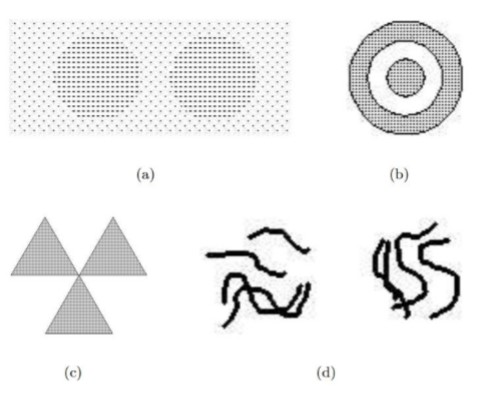
\includegraphics{wiki/1.1.jpg}
\caption{1.1}
\end{figure}

\begin{enumerate}
\def\labelenumi{\arabic{enumi}.}
\tightlist
\item
  Fig a)

  \begin{enumerate}
  \def\labelenumii{\arabic{enumii}.}
  \tightlist
  \item
    2 clusters: The centers will be add the center of two circles and
    noises in the rectangle will be incorporated into clusters.
  \item
    1 cluster: Due to existance of noise between to circles, they will
    be merged into a single cluster.
  \item
    2 clusters: 2 circles as the only dense area will be chosen as
    clusters and noises will be detected to separated from clusters. *
  \end{enumerate}
\item
  Fig b)

  \begin{enumerate}
  \def\labelenumii{\arabic{enumii}.}
  \tightlist
  \item
    1 cluster: The center will be at the center of concentric area of
    both circles otherwise, outer circle will be considered as noise.
  \item
    2 clusters: Each ring will represent a separate cluster. *
  \item
    2 clusters: Each ring will represent a separate cluster as they are
    dense w.r.t. their neighbors. * PS. result of 2 and 3 would be
    similar due to non-existance of noise.
  \end{enumerate}
\item
  Fig c)

  \begin{enumerate}
  \def\labelenumii{\arabic{enumii}.}
  \tightlist
  \item
    1 or 3 clusters:

    \begin{enumerate}
    \def\labelenumiii{\arabic{enumiii}.}
    \tightlist
    \item
      1 cluster where center is the joint point.
    \item
      3 is the better answer which each center will be at the center of
      each triangle to maintain equal distance. *
    \end{enumerate}
  \item
    1 cluster: The joint area of three triangle will cause it
  \item
    1 or 3 clusters:

    \begin{enumerate}
    \def\labelenumiii{\arabic{enumiii}.}
    \tightlist
    \item
      1 cluster: If the triangles \emph{overlap} and the joint area is
      not a single point, then it is possible w.r.t. to different
      paramters.
    \item
      3 clusters: Each triangle is the most dense area.
    \end{enumerate}
  \end{enumerate}
\item
  Fig d)

  \begin{enumerate}
  \def\labelenumii{\arabic{enumii}.}
  \tightlist
  \item
    2 clusters: Each center will be near the center of a circle
    containig all the threads.
  \item
    4 or 5 clusters: Assume that threads with joint area as a separate
    cluster, then left side will have 2 or 3 clusters and right side 2
    clusters.
  \item
    2 or 3 clusters: If we choose min distance large enough, then 2 if
    not it can be 3 as there is a considerable distance between threads
    in left side but best answer would be 2. *
  \end{enumerate}
\end{enumerate}

    \hypertarget{section}{%
\subsection{2}\label{section}}

Let's say we have two binary vectors:

\texttt{M11} represents the total number of attributes where A and B
both have a value of 1. \texttt{M01} represents the total number of
attributes where the attribute of A is 0 and the attribute of B is 1.
\texttt{M10} represents the total number of attributes where the
attribute of A is 1 and the attribute of B is 0. \texttt{M00} represents
the total number of attributes where A and B both have a value of 0.

Jaccard:

\begin{figure}
\centering
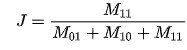
\includegraphics{wiki/2.1.jpg}
\caption{2.1}
\end{figure}

SMC:

\begin{figure}
\centering
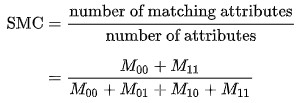
\includegraphics{wiki/2.2.jpg}
\caption{2.2}
\end{figure}

As we can see, the only difference between SMC and Jaccard is that SMC
adds \texttt{M00} in numinator and denominator.

On the other side, if we define Hamming \emph{similiarty} (1 - Hamming
Distance) as the number of similar bits, the
\texttt{Hamming\ /\ len(vector)\ =\ SMC}. Hence, \texttt{SMC} is
normalized \texttt{Hamming}. Note that the Hamming distance between two
equal-length strings of symbols is the number of positions at which the
corresponding symbols are different.

And Also, we can define Cosine similarity as normalized dot product
which demonstrates similarities of 1s in vectors which is \texttt{M11}
where is holding the definition of Jaccard.

\begin{figure}
\centering
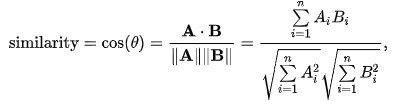
\includegraphics{wiki/2.3.jpg}
\caption{2.3}
\end{figure}

    \hypertarget{section}{%
\subsection{3}\label{section}}

\begin{figure}
\centering
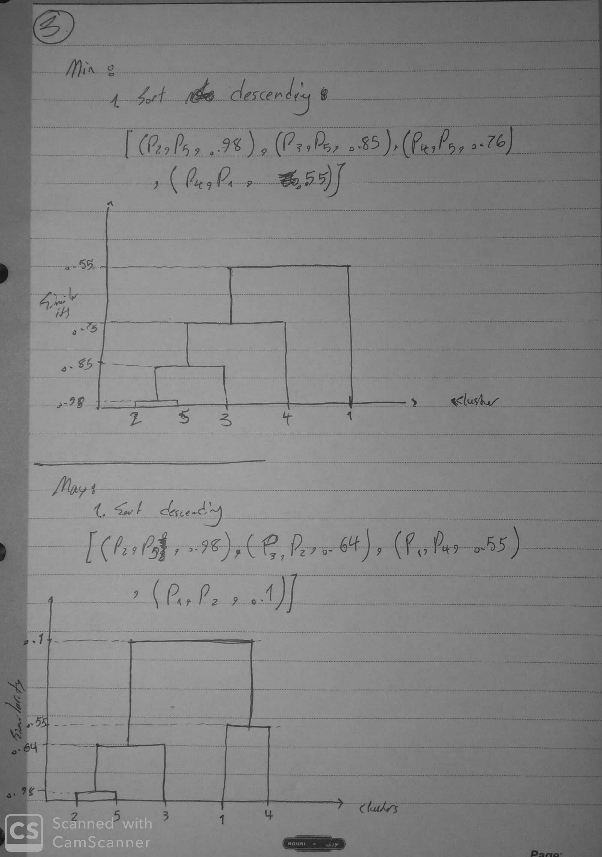
\includegraphics{wiki/3_.jpg}
\caption{3}
\end{figure}

    \hypertarget{section}{%
\subsection{4}\label{section}}

The answer would be NO. The main point again is the distance metric
which in our case we assume it is Euclidean distance. In this scenario,
euclidean distance will produce higher results for attributes with
higher mean or variance toward particular magnitude of space such as
skewness.

If we do not normalized our data, then one variable with higher
variance/mean tend to have higher impact on the result and so the
clustering is biased toward that particular variable. By removing this
bias/variance using normalization, we can ensure that all attributes are
incroporated with same proportion.

Also, Kmeans using euclidean distance tends to create circular clusters
so if data has skewness then normalization will have much higher impact
as normalized data is distributed around center of coordinate (mean=0,
variance=1) which is not true about unnormalized data.

Note that in all of interpretation, different mean and variance for
different attributes mean different physical/real world intrepretation.
If two attributes have different mean/variance but are in same domain,
then standardazation might not be necessary as the one with higher/lower
mean/variance may have more/lower importance.

In the end, all of these views depend on the prespective of tasks but
normally, normalization helps numerical stability of algorithm.

    \hypertarget{section}{%
\subsection{5}\label{section}}

\begin{enumerate}
\def\labelenumi{\arabic{enumi}.}
\tightlist
\item
  Robustness to noise:

  \begin{enumerate}
  \def\labelenumii{\arabic{enumii}.}
  \tightlist
  \item
    Single Link: If we look at the definition which is merging two
    clusters whose two closest points have the smallet distance, we can
    find out that this approach do not care about largest distances
    which directly corresponds to the outliers and noises. Hence, this
    approach is not robust to noises.
  \item
    Complete Link: Again, its definition states that we only merge two
    clusters where merger cluster has smaller diameter and if we try to
    demonstrate outliers and noises, we will see them in a distance away
    from the dense diameter of a cluster, then this approach works as a
    threshold and removes most of the noises and outliers.
  \item
    Average Link is a combo of two previously mentioned approachs which
    can be controlled to have robustness to noise w.r.t. complete link
    attribute or tendency of single link approach which try to construct
    clusters in form of long threads.
  \end{enumerate}
\item
  Time Complexity:

  \begin{enumerate}
  \def\labelenumii{\arabic{enumii}.}
  \tightlist
  \item
    Single Link: In this scenario, in each step we compute a distance
    between clusters which is \texttt{n\^{}2}. Then we one list of
    smallest distances for each cluster for merging time which takes
    \texttt{n} to be updated. Also, in each step, we need to update
    proximity matrix which takes \texttt{n} too. But all of this can be
    done while distances are computing and then sequentially so worst
    case would be \texttt{O(n\^{}2)}.
  \item
    Complete Link: The main difference from Single link is that in
    Single Link if \texttt{i} and \texttt{j} are merged, then the best
    merger for \texttt{k} is either \texttt{i} and \texttt{j} and that
    is why we only need to save smallest distance for each cluster
    rather than a list for each cluster. This is not true for complete
    link because any cluster rather than \texttt{i} or \texttt{j} can be
    best merger for \texttt{k}, hence we need to maintain a sorted list
    of smallest distances for each cluster which takes \texttt{log\ n}
    time so we have \texttt{O(log(n).n\^{}2)}.
  \item
    Average Groupd Link: Based on image, same time complexity can be
    considered for Average Group Link
  \end{enumerate}
\end{enumerate}

\begin{figure}
\centering
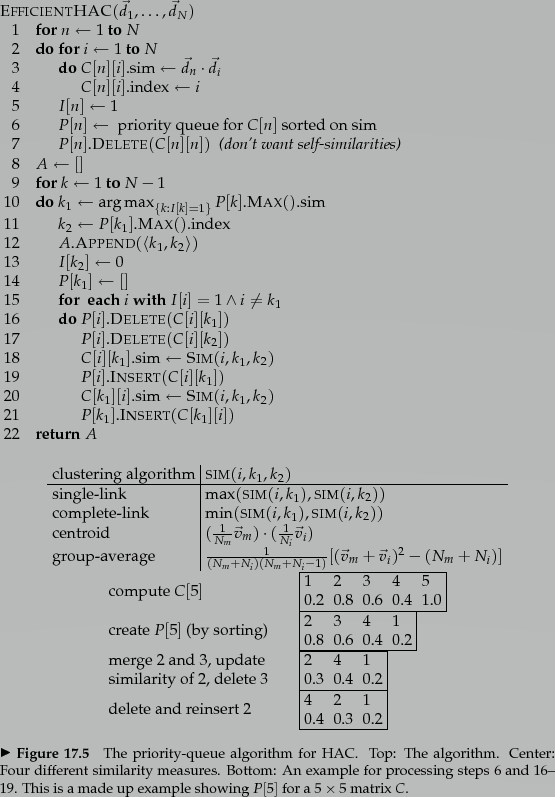
\includegraphics{wiki/5.jpg}
\caption{5}
\end{figure}

ref: \href{http://informationretrieval.org/}{Introduction to Information
Retrieval}, By Christopher D. Manning, Prabhakar Raghavan \& Hinrich
Schütze

    \hypertarget{dbscan}{%
\subsection{DBSCAN}\label{dbscan}}

    \begin{Verbatim}[commandchars=\\\{\}]
{\color{incolor}In [{\color{incolor}2}]:} \PY{k+kn}{import} \PY{n+nn}{numpy} \PY{k}{as} \PY{n+nn}{np}
        \PY{k+kn}{import} \PY{n+nn}{pandas} \PY{k}{as} \PY{n+nn}{pd}
        \PY{k+kn}{from} \PY{n+nn}{copy} \PY{k}{import} \PY{n}{deepcopy}
        \PY{k+kn}{import} \PY{n+nn}{matplotlib}\PY{n+nn}{.}\PY{n+nn}{pyplot} \PY{k}{as} \PY{n+nn}{plt}
        
        \PY{k+kn}{from} \PY{n+nn}{sklearn}\PY{n+nn}{.}\PY{n+nn}{metrics}\PY{n+nn}{.}\PY{n+nn}{pairwise} \PY{k}{import} \PY{n}{euclidean\PYZus{}distances}
        \PY{k+kn}{from} \PY{n+nn}{sklearn} \PY{k}{import} \PY{n}{cluster}
\end{Verbatim}


    \begin{Verbatim}[commandchars=\\\{\}]
{\color{incolor}In [{\color{incolor}5}]:} \PY{n}{data} \PY{o}{=} \PY{n}{pd}\PY{o}{.}\PY{n}{read\PYZus{}csv}\PY{p}{(}\PY{l+s+s1}{\PYZsq{}}\PY{l+s+s1}{../data/data.csv}\PY{l+s+s1}{\PYZsq{}}\PY{p}{,} \PY{n}{header}\PY{o}{=}\PY{k+kc}{None}\PY{p}{)}
        \PY{n+nb}{print}\PY{p}{(}\PY{l+s+s1}{\PYZsq{}}\PY{l+s+s1}{Number of samples: }\PY{l+s+s1}{\PYZsq{}}\PY{p}{,} \PY{n+nb}{len}\PY{p}{(}\PY{n}{data}\PY{p}{)}\PY{p}{)}
        \PY{n}{data}\PY{o}{.}\PY{n}{plot}\PY{o}{.}\PY{n}{scatter}\PY{p}{(}\PY{l+m+mi}{0}\PY{p}{,} \PY{l+m+mi}{1}\PY{p}{,} \PY{n}{figsize}\PY{o}{=}\PY{p}{(}\PY{l+m+mi}{15}\PY{p}{,} \PY{l+m+mi}{10}\PY{p}{)}\PY{p}{)}
        \PY{n}{plt}\PY{o}{.}\PY{n}{show}\PY{p}{(}\PY{p}{)}
        
        \PY{n}{data} \PY{o}{=} \PY{n}{data}\PY{o}{.}\PY{n}{values}
\end{Verbatim}


    \begin{Verbatim}[commandchars=\\\{\}]
Number of samples:  788

    \end{Verbatim}

    \begin{center}
    \adjustimage{max size={0.9\linewidth}{0.9\paperheight}}{output_8_1.png}
    \end{center}
    { \hspace*{\fill} \\}
    
    \begin{Verbatim}[commandchars=\\\{\}]
{\color{incolor}In [{\color{incolor}7}]:} \PY{n}{mean} \PY{o}{=} \PY{n}{data}\PY{o}{.}\PY{n}{mean}\PY{p}{(}\PY{p}{)}
        \PY{n}{std} \PY{o}{=} \PY{n}{data}\PY{o}{.}\PY{n}{std}\PY{p}{(}\PY{p}{)}
        \PY{n}{data} \PY{o}{=} \PY{p}{(}\PY{n}{data} \PY{o}{\PYZhy{}} \PY{n}{mean}\PY{p}{)} \PY{o}{/} \PY{n}{std}
\end{Verbatim}


    \begin{Verbatim}[commandchars=\\\{\}]
{\color{incolor}In [{\color{incolor}8}]:} \PY{k}{class} \PY{n+nc}{DBSCAN}\PY{p}{:}
            \PY{k}{def} \PY{n+nf}{\PYZus{}\PYZus{}init\PYZus{}\PYZus{}}\PY{p}{(}\PY{n+nb+bp}{self}\PY{p}{,} \PY{n}{min\PYZus{}samples}\PY{p}{,} \PY{n}{eps}\PY{p}{)}\PY{p}{:}
                \PY{l+s+sd}{\PYZdq{}\PYZdq{}\PYZdq{}}
        \PY{l+s+sd}{        Constructs DBSCAN given parameters of neighborhood}
        
        \PY{l+s+sd}{        :param min\PYZus{}samples: Minimum samples within eps radius to be consider as a core point}
        \PY{l+s+sd}{        :param eps: Radius of core point}
        \PY{l+s+sd}{        \PYZdq{}\PYZdq{}\PYZdq{}}
                \PY{n+nb+bp}{self}\PY{o}{.}\PY{n}{min\PYZus{}samples} \PY{o}{=} \PY{n}{min\PYZus{}samples}
                \PY{n+nb+bp}{self}\PY{o}{.}\PY{n}{eps} \PY{o}{=} \PY{n}{eps}
        
                \PY{n+nb+bp}{self}\PY{o}{.}\PY{n}{labels} \PY{o}{=} \PY{k+kc}{None}  \PY{c+c1}{\PYZsh{} \PYZsq{}0\PYZsq{}: Haven\PYZsq{}t processed, \PYZsq{}\PYZhy{}1\PYZsq{}: noise, \PYZsq{}C\PYZsq{}: cluster number}
                \PY{n+nb+bp}{self}\PY{o}{.}\PY{n}{core\PYZus{}points} \PY{o}{=} \PY{k+kc}{None}
        
            \PY{k}{def} \PY{n+nf}{fit\PYZus{}predict}\PY{p}{(}\PY{n+nb+bp}{self}\PY{p}{,} \PY{n}{x}\PY{p}{,} \PY{o}{*}\PY{n}{args}\PY{p}{,} \PY{o}{*}\PY{o}{*}\PY{n}{kwargs}\PY{p}{)}\PY{p}{:}
                \PY{l+s+sd}{\PYZdq{}\PYZdq{}\PYZdq{}}
        \PY{l+s+sd}{        Fits the data using DBSCAN and returns labels and core points}
        \PY{l+s+sd}{        Order of data matter!}
        
        \PY{l+s+sd}{        Algorithm:}
        \PY{l+s+sd}{            1. Consider a list of points that have not been seen yet}
        \PY{l+s+sd}{            2. Read an arbitrary point until there is no unseen point left}
        \PY{l+s+sd}{            3. If there are at least ``min\PYZus{}samples`` points within a radius of ``eps``}
        \PY{l+s+sd}{                then all these points are from same cluster}
        \PY{l+s+sd}{            4. Expand this cluster for its all core points for all neighbors}
        \PY{l+s+sd}{            5. Repeat}
        
        \PY{l+s+sd}{        :param x: N\PYZhy{}dimensional numpy array}
        
        \PY{l+s+sd}{        :return: A tuple of labels of each point and index of core points}
        \PY{l+s+sd}{            where label=\PYZhy{}1 corresponds to noise data and label=N N\PYZgt{}=1 demonstrates cluster label}
        \PY{l+s+sd}{        \PYZdq{}\PYZdq{}\PYZdq{}}
        
                \PY{n+nb+bp}{self}\PY{o}{.}\PY{n}{labels} \PY{o}{=} \PY{n}{np}\PY{o}{.}\PY{n}{zeros}\PY{p}{(}\PY{p}{(}\PY{n+nb}{len}\PY{p}{(}\PY{n}{x}\PY{p}{)}\PY{p}{,}\PY{p}{)}\PY{p}{)}
                \PY{n+nb+bp}{self}\PY{o}{.}\PY{n}{core\PYZus{}points} \PY{o}{=} \PY{n}{np}\PY{o}{.}\PY{n}{zeros}\PY{p}{(}\PY{p}{(}\PY{n+nb}{len}\PY{p}{(}\PY{n}{x}\PY{p}{)}\PY{p}{,}\PY{p}{)}\PY{p}{)}
                \PY{n}{current\PYZus{}cluster} \PY{o}{=} \PY{l+m+mi}{1}  \PY{c+c1}{\PYZsh{} we use 1\PYZhy{}\PYZgt{}inf}
        
                \PY{k}{for} \PY{n}{pnt} \PY{o+ow}{in} \PY{n+nb}{range}\PY{p}{(}\PY{n+nb}{len}\PY{p}{(}\PY{n}{x}\PY{p}{)}\PY{p}{)}\PY{p}{:}
                    \PY{c+c1}{\PYZsh{} if self.labels[pnt] == \PYZhy{}1 or self.labels[pnt] \PYZgt{}= 1:}
                    \PY{k}{if} \PY{n+nb+bp}{self}\PY{o}{.}\PY{n}{labels}\PY{p}{[}\PY{n}{pnt}\PY{p}{]} \PY{o}{==} \PY{l+m+mi}{0}\PY{p}{:}
                        \PY{n}{neighbor\PYZus{}indices} \PY{o}{=} \PY{n+nb+bp}{self}\PY{o}{.}\PY{n}{\PYZus{}\PYZus{}nearest\PYZus{}neighbors}\PY{p}{(}\PY{n}{x}\PY{p}{,} \PY{n}{x}\PY{p}{[}\PY{n}{pnt}\PY{p}{]}\PY{p}{)}
        
                        \PY{k}{if} \PY{n+nb}{len}\PY{p}{(}\PY{n}{neighbor\PYZus{}indices}\PY{p}{)} \PY{o}{\PYZgt{}}\PY{o}{=} \PY{n+nb+bp}{self}\PY{o}{.}\PY{n}{min\PYZus{}samples}\PY{p}{:}
                            \PY{n+nb+bp}{self}\PY{o}{.}\PY{n}{\PYZus{}\PYZus{}expand}\PY{p}{(}\PY{n}{x}\PY{p}{,} \PY{n}{pnt}\PY{p}{,} \PY{n}{current\PYZus{}cluster}\PY{p}{)}
                            \PY{n}{current\PYZus{}cluster} \PY{o}{+}\PY{o}{=} \PY{l+m+mi}{1}
                        \PY{k}{else}\PY{p}{:}  \PY{c+c1}{\PYZsh{} noise/outlier scenario}
                            \PY{n+nb+bp}{self}\PY{o}{.}\PY{n}{labels}\PY{p}{[}\PY{n}{pnt}\PY{p}{]} \PY{o}{=} \PY{o}{\PYZhy{}}\PY{l+m+mi}{1}
                \PY{k}{return} \PY{n+nb+bp}{self}\PY{o}{.}\PY{n}{labels}\PY{p}{,} \PY{n+nb+bp}{self}\PY{o}{.}\PY{n}{core\PYZus{}points}
        
            \PY{k}{def} \PY{n+nf}{\PYZus{}\PYZus{}nearest\PYZus{}neighbors}\PY{p}{(}\PY{n+nb+bp}{self}\PY{p}{,} \PY{n}{data}\PY{p}{,} \PY{n}{point}\PY{p}{)}\PY{p}{:}
                \PY{l+s+sd}{\PYZdq{}\PYZdq{}\PYZdq{}}
        \PY{l+s+sd}{        Finds points near to the point ``point`` within the range of ``eps``}
        
        \PY{l+s+sd}{        :param point: A point}
        \PY{l+s+sd}{        :param: All points}
        
        \PY{l+s+sd}{        :return: Indices of nearest neighbor points}
        \PY{l+s+sd}{        \PYZdq{}\PYZdq{}\PYZdq{}}
                \PY{n}{distances} \PY{o}{=} \PY{n}{euclidean\PYZus{}distances}\PY{p}{(}\PY{n}{data}\PY{p}{,} \PY{n}{point}\PY{o}{.}\PY{n}{reshape}\PY{p}{(}\PY{l+m+mi}{1}\PY{p}{,} \PY{o}{\PYZhy{}}\PY{l+m+mi}{1}\PY{p}{)}\PY{p}{)}
                \PY{n}{neighbors} \PY{o}{=} \PY{n}{distances} \PY{o}{\PYZlt{}}\PY{o}{=} \PY{n+nb+bp}{self}\PY{o}{.}\PY{n}{eps}
                \PY{n}{topk} \PY{o}{=} \PY{n}{np}\PY{o}{.}\PY{n}{argsort}\PY{p}{(}\PY{n}{distances}\PY{p}{,} \PY{n}{axis}\PY{o}{=}\PY{l+m+mi}{0}\PY{p}{)}
                \PY{n}{neighbors\PYZus{}idx} \PY{o}{=} \PY{n}{np}\PY{o}{.}\PY{n}{max}\PY{p}{(}\PY{n}{neighbors}\PY{p}{[}\PY{n}{topk}\PY{p}{]}\PY{o}{.}\PY{n}{nonzero}\PY{p}{(}\PY{p}{)}\PY{p}{[}\PY{l+m+mi}{0}\PY{p}{]}\PY{p}{)} \PY{o}{+} \PY{l+m+mi}{1}
                \PY{k}{return} \PY{n}{topk}\PY{p}{[}\PY{p}{:}\PY{n}{neighbors\PYZus{}idx}\PY{p}{]}\PY{o}{.}\PY{n}{flatten}\PY{p}{(}\PY{p}{)}
        
            \PY{k}{def} \PY{n+nf}{\PYZus{}\PYZus{}expand}\PY{p}{(}\PY{n+nb+bp}{self}\PY{p}{,} \PY{n}{data}\PY{p}{,} \PY{n}{point\PYZus{}idx}\PY{p}{,} \PY{n}{current\PYZus{}cluster}\PY{p}{)}\PY{p}{:}
                \PY{l+s+sd}{\PYZdq{}\PYZdq{}\PYZdq{}}
        \PY{l+s+sd}{        Expands ``current\PYZus{}cluster`` using given point w.r.t. ``eps`` and ``min\PYZus{}samples``}
        \PY{l+s+sd}{        Algorithm:}
        \PY{l+s+sd}{            1. Get a point as the start point for ``current\PYZus{}cluster``}
        \PY{l+s+sd}{            2. Get its neighbors and go through them one by one using queue logic}
        \PY{l+s+sd}{            3. If the neighbor is noise, then add it to the current cluster, if it is unseen, get all its neighbors}
        \PY{l+s+sd}{                 then add them to the list of neighbors of original point}
        \PY{l+s+sd}{            4. Repeat step 2 and 3 until all points in the list of neighbors are processed.}
        
        \PY{l+s+sd}{        :param data: Whole data to be clustered}
        \PY{l+s+sd}{        :param point\PYZus{}idx: The index of a point of the current cluster as the start point for expansion}
        \PY{l+s+sd}{        :param current\PYZus{}cluster: The label of current cluster}
        \PY{l+s+sd}{        :return: None}
        \PY{l+s+sd}{        \PYZdq{}\PYZdq{}\PYZdq{}}
        
                \PY{n+nb+bp}{self}\PY{o}{.}\PY{n}{labels}\PY{p}{[}\PY{n}{point\PYZus{}idx}\PY{p}{]} \PY{o}{=} \PY{n}{current\PYZus{}cluster}
                \PY{n}{neighbors\PYZus{}indices} \PY{o}{=} \PY{n}{deepcopy}\PY{p}{(}\PY{n+nb+bp}{self}\PY{o}{.}\PY{n}{\PYZus{}\PYZus{}nearest\PYZus{}neighbors}\PY{p}{(}\PY{n}{data}\PY{p}{,} \PY{n}{data}\PY{p}{[}\PY{n}{point\PYZus{}idx}\PY{p}{]}\PY{p}{)}\PY{p}{)}
        
                \PY{k}{while} \PY{n+nb}{len}\PY{p}{(}\PY{n}{neighbors\PYZus{}indices}\PY{p}{)} \PY{o}{\PYZgt{}} \PY{l+m+mi}{0}\PY{p}{:}
                    \PY{n}{neighbor\PYZus{}point} \PY{o}{=} \PY{n}{neighbors\PYZus{}indices}\PY{p}{[}\PY{l+m+mi}{0}\PY{p}{]}
                    \PY{n}{neighbors\PYZus{}indices} \PY{o}{=} \PY{n}{np}\PY{o}{.}\PY{n}{delete}\PY{p}{(}\PY{n}{neighbors\PYZus{}indices}\PY{p}{,} \PY{l+m+mi}{0}\PY{p}{,} \PY{l+m+mi}{0}\PY{p}{)}
                    \PY{k}{if} \PY{n+nb+bp}{self}\PY{o}{.}\PY{n}{labels}\PY{p}{[}\PY{n}{neighbor\PYZus{}point}\PY{p}{]} \PY{o}{==} \PY{o}{\PYZhy{}}\PY{l+m+mi}{1}\PY{p}{:}
                        \PY{n+nb+bp}{self}\PY{o}{.}\PY{n}{labels}\PY{p}{[}\PY{n}{neighbor\PYZus{}point}\PY{p}{]} \PY{o}{=} \PY{n}{current\PYZus{}cluster}
                    \PY{k}{elif} \PY{n+nb+bp}{self}\PY{o}{.}\PY{n}{labels}\PY{p}{[}\PY{n}{neighbor\PYZus{}point}\PY{p}{]} \PY{o}{==} \PY{l+m+mi}{0}\PY{p}{:}
                        \PY{n+nb+bp}{self}\PY{o}{.}\PY{n}{labels}\PY{p}{[}\PY{n}{neighbor\PYZus{}point}\PY{p}{]} \PY{o}{=} \PY{n}{current\PYZus{}cluster}
                        \PY{n}{neighbors\PYZus{}indices\PYZus{}neighbor\PYZus{}point} \PY{o}{=} \PY{n+nb+bp}{self}\PY{o}{.}\PY{n}{\PYZus{}\PYZus{}nearest\PYZus{}neighbors}\PY{p}{(}\PY{n}{data}\PY{p}{,} \PY{n}{data}\PY{p}{[}\PY{n}{neighbor\PYZus{}point}\PY{p}{]}\PY{p}{)}
                        \PY{k}{if} \PY{n+nb}{len}\PY{p}{(}\PY{n}{neighbors\PYZus{}indices\PYZus{}neighbor\PYZus{}point}\PY{p}{)} \PY{o}{\PYZgt{}}\PY{o}{=} \PY{n+nb+bp}{self}\PY{o}{.}\PY{n}{min\PYZus{}samples}\PY{p}{:}
                            \PY{n}{neighbors\PYZus{}indices} \PY{o}{=} \PY{n}{np}\PY{o}{.}\PY{n}{concatenate}\PY{p}{(}\PY{p}{(}\PY{n}{neighbors\PYZus{}indices}\PY{p}{,} \PY{n}{neighbors\PYZus{}indices\PYZus{}neighbor\PYZus{}point}\PY{p}{)}\PY{p}{)}
                            \PY{n+nb+bp}{self}\PY{o}{.}\PY{n}{core\PYZus{}points}\PY{p}{[}\PY{n}{neighbor\PYZus{}point}\PY{p}{]} \PY{o}{=} \PY{l+m+mi}{1}
\end{Verbatim}


    \begin{Verbatim}[commandchars=\\\{\}]
{\color{incolor}In [{\color{incolor}9}]:} \PY{n}{parameters} \PY{o}{=} \PY{p}{\PYZob{}}\PY{l+s+s1}{\PYZsq{}}\PY{l+s+s1}{eps}\PY{l+s+s1}{\PYZsq{}}\PY{p}{:} \PY{p}{[}\PY{l+m+mf}{0.25}\PY{p}{,} \PY{l+m+mf}{0.3}\PY{p}{,} \PY{l+m+mf}{0.35}\PY{p}{,} \PY{l+m+mf}{0.4}\PY{p}{]}\PY{p}{,} \PY{l+s+s1}{\PYZsq{}}\PY{l+s+s1}{min\PYZus{}samples}\PY{l+s+s1}{\PYZsq{}}\PY{p}{:} \PY{p}{[}\PY{l+m+mi}{3}\PY{p}{,} \PY{l+m+mi}{4}\PY{p}{,} \PY{l+m+mi}{5}\PY{p}{,} \PY{l+m+mi}{6}\PY{p}{,} \PY{l+m+mi}{7}\PY{p}{,} \PY{l+m+mi}{10}\PY{p}{]}\PY{p}{\PYZcb{}}
        
        \PY{n}{plt}\PY{o}{.}\PY{n}{figure}\PY{p}{(}\PY{n}{figsize}\PY{o}{=}\PY{p}{(}\PY{l+m+mi}{20}\PY{p}{,} \PY{l+m+mi}{9}\PY{p}{)}\PY{p}{)}
        \PY{n}{i} \PY{o}{=} \PY{l+m+mi}{0}
        \PY{k}{for} \PY{n}{dist} \PY{o+ow}{in} \PY{n}{parameters}\PY{p}{[}\PY{l+s+s1}{\PYZsq{}}\PY{l+s+s1}{eps}\PY{l+s+s1}{\PYZsq{}}\PY{p}{]}\PY{p}{:}
            \PY{k}{for} \PY{n}{min\PYZus{}pnt} \PY{o+ow}{in} \PY{n}{parameters}\PY{p}{[}\PY{l+s+s1}{\PYZsq{}}\PY{l+s+s1}{min\PYZus{}samples}\PY{l+s+s1}{\PYZsq{}}\PY{p}{]}\PY{p}{:}
                \PY{n}{dbscan} \PY{o}{=} \PY{n}{DBSCAN}\PY{p}{(}\PY{n}{min\PYZus{}samples}\PY{o}{=}\PY{n}{min\PYZus{}pnt}\PY{p}{,} \PY{n}{eps}\PY{o}{=}\PY{n}{dist}\PY{p}{)}
                \PY{n}{y\PYZus{}dbscan}\PY{p}{,} \PY{n}{\PYZus{}} \PY{o}{=} \PY{n}{dbscan}\PY{o}{.}\PY{n}{fit\PYZus{}predict}\PY{p}{(}\PY{n}{data}\PY{p}{)}
                \PY{n}{plt}\PY{o}{.}\PY{n}{subplot}\PY{p}{(}\PY{n+nb}{len}\PY{p}{(}\PY{n}{parameters}\PY{p}{[}\PY{l+s+s1}{\PYZsq{}}\PY{l+s+s1}{eps}\PY{l+s+s1}{\PYZsq{}}\PY{p}{]}\PY{p}{)}\PY{p}{,} \PY{n+nb}{len}\PY{p}{(}\PY{n}{parameters}\PY{p}{[}\PY{l+s+s1}{\PYZsq{}}\PY{l+s+s1}{min\PYZus{}samples}\PY{l+s+s1}{\PYZsq{}}\PY{p}{]}\PY{p}{)}\PY{p}{,} \PY{n}{i}\PY{o}{+}\PY{l+m+mi}{1}\PY{p}{)}
                \PY{n}{i} \PY{o}{+}\PY{o}{=} \PY{l+m+mi}{1}
                \PY{n}{plt}\PY{o}{.}\PY{n}{scatter}\PY{p}{(}\PY{n}{data}\PY{p}{[}\PY{p}{:}\PY{p}{,} \PY{l+m+mi}{0}\PY{p}{]}\PY{p}{,} \PY{n}{data}\PY{p}{[}\PY{p}{:}\PY{p}{,} \PY{l+m+mi}{1}\PY{p}{]}\PY{p}{,} \PY{n}{c}\PY{o}{=}\PY{n}{y\PYZus{}dbscan}\PY{p}{,} \PY{n}{s}\PY{o}{=}\PY{l+m+mi}{50}\PY{p}{,} \PY{n}{cmap}\PY{o}{=}\PY{l+s+s1}{\PYZsq{}}\PY{l+s+s1}{viridis}\PY{l+s+s1}{\PYZsq{}}\PY{p}{,} \PY{n}{label}\PY{o}{=}\PY{n}{np}\PY{o}{.}\PY{n}{unique}\PY{p}{(}\PY{n}{y\PYZus{}dbscan}\PY{p}{)}\PY{p}{)}
                \PY{n}{plt}\PY{o}{.}\PY{n}{legend}\PY{p}{(}\PY{p}{)}
        \PY{n}{plt}\PY{o}{.}\PY{n}{show}\PY{p}{(}\PY{p}{)}
\end{Verbatim}


    \begin{center}
    \adjustimage{max size={0.9\linewidth}{0.9\paperheight}}{output_11_0.png}
    \end{center}
    { \hspace*{\fill} \\}
    
    \begin{Verbatim}[commandchars=\\\{\}]
{\color{incolor}In [{\color{incolor}12}]:} \PY{n}{plt}\PY{o}{.}\PY{n}{figure}\PY{p}{(}\PY{n}{figsize}\PY{o}{=}\PY{p}{(}\PY{l+m+mi}{9}\PY{p}{,} \PY{l+m+mi}{6}\PY{p}{)}\PY{p}{)}
         \PY{n}{dbscan} \PY{o}{=} \PY{n}{DBSCAN}\PY{p}{(}\PY{n}{min\PYZus{}samples}\PY{o}{=}\PY{l+m+mi}{5}\PY{p}{,} \PY{n}{eps}\PY{o}{=}\PY{l+m+mf}{0.3}\PY{p}{)}
         \PY{n}{y\PYZus{}dbscan}\PY{p}{,} \PY{n}{centers} \PY{o}{=} \PY{n}{dbscan}\PY{o}{.}\PY{n}{fit\PYZus{}predict}\PY{p}{(}\PY{n}{data}\PY{p}{)}
         \PY{n}{plt}\PY{o}{.}\PY{n}{scatter}\PY{p}{(}\PY{n}{data}\PY{p}{[}\PY{p}{:}\PY{p}{,} \PY{l+m+mi}{0}\PY{p}{]}\PY{p}{,} \PY{n}{data}\PY{p}{[}\PY{p}{:}\PY{p}{,} \PY{l+m+mi}{1}\PY{p}{]}\PY{p}{,} \PY{n}{c}\PY{o}{=}\PY{n}{y\PYZus{}dbscan}\PY{p}{,} \PY{n}{s}\PY{o}{=}\PY{l+m+mi}{50}\PY{p}{,} \PY{n}{cmap}\PY{o}{=}\PY{l+s+s1}{\PYZsq{}}\PY{l+s+s1}{viridis}\PY{l+s+s1}{\PYZsq{}}\PY{p}{,} \PY{n}{label}\PY{o}{=}\PY{n}{np}\PY{o}{.}\PY{n}{unique}\PY{p}{(}\PY{n}{y\PYZus{}dbscan}\PY{p}{)}\PY{p}{)}
         \PY{n}{plt}\PY{o}{.}\PY{n}{legend}\PY{p}{(}\PY{p}{)}
         \PY{n}{plt}\PY{o}{.}\PY{n}{show}\PY{p}{(}\PY{p}{)}
\end{Verbatim}


    \begin{center}
    \adjustimage{max size={0.9\linewidth}{0.9\paperheight}}{output_12_0.png}
    \end{center}
    { \hspace*{\fill} \\}
    
    \hypertarget{kmeans}{%
\subsection{KMeans}\label{kmeans}}

    \begin{Verbatim}[commandchars=\\\{\}]
{\color{incolor}In [{\color{incolor}1}]:} \PY{k+kn}{import} \PY{n+nn}{numpy} \PY{k}{as} \PY{n+nn}{np}
        \PY{k+kn}{import} \PY{n+nn}{pandas} \PY{k}{as} \PY{n+nn}{pd}
        \PY{k+kn}{import} \PY{n+nn}{matplotlib}\PY{n+nn}{.}\PY{n+nn}{pyplot} \PY{k}{as} \PY{n+nn}{plt}
        \PY{o}{\PYZpc{}}\PY{k}{matplotlib} inline
\end{Verbatim}


    \begin{Verbatim}[commandchars=\\\{\}]
{\color{incolor}In [{\color{incolor}3}]:} \PY{n}{data} \PY{o}{=} \PY{n}{pd}\PY{o}{.}\PY{n}{read\PYZus{}csv}\PY{p}{(}\PY{l+s+s1}{\PYZsq{}}\PY{l+s+s1}{../data/data.csv}\PY{l+s+s1}{\PYZsq{}}\PY{p}{,} \PY{n}{header}\PY{o}{=}\PY{k+kc}{None}\PY{p}{)}
        \PY{n+nb}{print}\PY{p}{(}\PY{l+s+s1}{\PYZsq{}}\PY{l+s+s1}{Number of samples: }\PY{l+s+s1}{\PYZsq{}}\PY{p}{,}\PY{n+nb}{len}\PY{p}{(}\PY{n}{data}\PY{p}{)}\PY{p}{)}
        \PY{n}{data}\PY{o}{.}\PY{n}{plot}\PY{o}{.}\PY{n}{scatter}\PY{p}{(}\PY{l+m+mi}{0}\PY{p}{,} \PY{l+m+mi}{1}\PY{p}{,} \PY{n}{figsize}\PY{o}{=}\PY{p}{(}\PY{l+m+mi}{15}\PY{p}{,} \PY{l+m+mi}{10}\PY{p}{)}\PY{p}{)}
        \PY{n}{plt}\PY{o}{.}\PY{n}{show}\PY{p}{(}\PY{p}{)}
        
        \PY{n}{data} \PY{o}{=} \PY{n}{data}\PY{o}{.}\PY{n}{values}
\end{Verbatim}


    \begin{Verbatim}[commandchars=\\\{\}]
Number of samples:  788

    \end{Verbatim}

    \begin{center}
    \adjustimage{max size={0.9\linewidth}{0.9\paperheight}}{output_15_1.png}
    \end{center}
    { \hspace*{\fill} \\}
    
    \begin{Verbatim}[commandchars=\\\{\}]
{\color{incolor}In [{\color{incolor}4}]:} \PY{c+c1}{\PYZsh{} normalization}
        \PY{n}{mean} \PY{o}{=} \PY{n}{data}\PY{o}{.}\PY{n}{mean}\PY{p}{(}\PY{p}{)}
        \PY{n}{std} \PY{o}{=} \PY{n}{data}\PY{o}{.}\PY{n}{std}\PY{p}{(}\PY{p}{)}
        \PY{n}{data} \PY{o}{=} \PY{p}{(}\PY{n}{data} \PY{o}{\PYZhy{}} \PY{n}{mean}\PY{p}{)} \PY{o}{/} \PY{n}{std}
\end{Verbatim}


    \begin{Verbatim}[commandchars=\\\{\}]
{\color{incolor}In [{\color{incolor}19}]:} \PY{c+c1}{\PYZsh{} DBI}
         \PY{k+kn}{from} \PY{n+nn}{sklearn}\PY{n+nn}{.}\PY{n+nn}{metrics}\PY{n+nn}{.}\PY{n+nn}{pairwise} \PY{k}{import} \PY{n}{euclidean\PYZus{}distances}
         \PY{k+kn}{from} \PY{n+nn}{sklearn}\PY{n+nn}{.}\PY{n+nn}{metrics} \PY{k}{import} \PY{n}{make\PYZus{}scorer}
         
         \PY{k+kn}{from} \PY{n+nn}{sklearn}\PY{n+nn}{.}\PY{n+nn}{cluster} \PY{k}{import} \PY{n}{KMeans}
         
         \PY{k}{def} \PY{n+nf}{DB\PYZus{}loss\PYZus{}function}\PY{p}{(}\PY{n}{estimator}\PY{p}{,} \PY{n}{X}\PY{p}{,} \PY{n}{y\PYZus{}true}\PY{o}{=}\PY{k+kc}{None}\PY{p}{)}\PY{p}{:}
             \PY{l+s+sd}{\PYZdq{}\PYZdq{}\PYZdq{}}
         \PY{l+s+sd}{    Computes Davis\PYZhy{}Bolding Index for a fitted KMeans}
         
         \PY{l+s+sd}{    args:}
         \PY{l+s+sd}{        model: Fitted KMeans object}
         \PY{l+s+sd}{        x: input data for evaluation }
         \PY{l+s+sd}{    \PYZdq{}\PYZdq{}\PYZdq{}}
             \PY{n}{preds} \PY{o}{=} \PY{n}{estimator}\PY{o}{.}\PY{n}{predict}\PY{p}{(}\PY{n}{X}\PY{p}{)}
             \PY{n}{n\PYZus{}clusters} \PY{o}{=} \PY{n+nb}{int}\PY{p}{(}\PY{n}{np}\PY{o}{.}\PY{n}{max}\PY{p}{(}\PY{n}{preds}\PY{p}{)}\PY{p}{)}\PY{o}{+}\PY{l+m+mi}{1}
         
             \PY{n}{db\PYZus{}values} \PY{o}{=} \PY{p}{[}\PY{p}{]}
             \PY{k}{for} \PY{n}{i} \PY{o+ow}{in} \PY{n+nb}{range}\PY{p}{(}\PY{n}{n\PYZus{}clusters}\PY{p}{)}\PY{p}{:}
                 \PY{k}{for} \PY{n}{j} \PY{o+ow}{in} \PY{n+nb}{range}\PY{p}{(}\PY{n}{i}\PY{o}{+}\PY{l+m+mi}{1}\PY{p}{,} \PY{n}{n\PYZus{}clusters}\PY{p}{)}\PY{p}{:}
                     \PY{n}{cluster\PYZus{}i} \PY{o}{=} \PY{n}{X}\PY{p}{[}\PY{n}{preds} \PY{o}{==} \PY{n}{i}\PY{p}{]}
                     \PY{n}{cluster\PYZus{}j} \PY{o}{=} \PY{n}{X}\PY{p}{[}\PY{n}{preds} \PY{o}{==} \PY{n}{j}\PY{p}{]}
                     
                     \PY{n}{avg\PYZus{}cluster\PYZus{}i} \PY{o}{=} \PY{l+m+mi}{2} \PY{o}{*} \PY{n}{np}\PY{o}{.}\PY{n}{sum}\PY{p}{(}\PY{n}{euclidean\PYZus{}distances}\PY{p}{(}\PY{n}{cluster\PYZus{}i}\PY{p}{,} \PY{n}{cluster\PYZus{}i}\PY{p}{)}\PY{p}{)} \PY{o}{/} \PY{n+nb}{len}\PY{p}{(}\PY{n}{cluster\PYZus{}i}\PY{p}{)}\PY{o}{*}\PY{p}{(}\PY{n+nb}{len}\PY{p}{(}\PY{n}{cluster\PYZus{}i}\PY{p}{)}\PY{o}{\PYZhy{}}\PY{l+m+mi}{1}\PY{p}{)}
                     \PY{n}{avg\PYZus{}cluster\PYZus{}j} \PY{o}{=} \PY{l+m+mi}{2} \PY{o}{*} \PY{n}{np}\PY{o}{.}\PY{n}{sum}\PY{p}{(}\PY{n}{euclidean\PYZus{}distances}\PY{p}{(}\PY{n}{cluster\PYZus{}j}\PY{p}{,} \PY{n}{cluster\PYZus{}j}\PY{p}{)}\PY{p}{)} \PY{o}{/} \PY{n+nb}{len}\PY{p}{(}\PY{n}{cluster\PYZus{}j}\PY{p}{)}\PY{o}{*}\PY{p}{(}\PY{n+nb}{len}\PY{p}{(}\PY{n}{cluster\PYZus{}j}\PY{p}{)}\PY{o}{\PYZhy{}}\PY{l+m+mi}{1}\PY{p}{)}
         
                     \PY{n}{u\PYZus{}cluster\PYZus{}i} \PY{o}{=} \PY{n}{np}\PY{o}{.}\PY{n}{sum}\PY{p}{(}\PY{n}{cluster\PYZus{}i}\PY{p}{,} \PY{n}{axis}\PY{o}{=}\PY{l+m+mi}{0}\PY{p}{)} \PY{o}{/} \PY{n+nb}{len}\PY{p}{(}\PY{n}{cluster\PYZus{}i}\PY{p}{)}
                     \PY{n}{u\PYZus{}cluster\PYZus{}j} \PY{o}{=} \PY{n}{np}\PY{o}{.}\PY{n}{sum}\PY{p}{(}\PY{n}{cluster\PYZus{}j}\PY{p}{,} \PY{n}{axis}\PY{o}{=}\PY{l+m+mi}{0}\PY{p}{)} \PY{o}{/} \PY{n+nb}{len}\PY{p}{(}\PY{n}{cluster\PYZus{}j}\PY{p}{)}
                     \PY{n}{db} \PY{o}{=} \PY{p}{(}\PY{n}{avg\PYZus{}cluster\PYZus{}i} \PY{o}{+} \PY{n}{avg\PYZus{}cluster\PYZus{}j}\PY{p}{)} \PY{o}{/} \PY{n}{np}\PY{o}{.}\PY{n}{sum}\PY{p}{(}\PY{n}{euclidean\PYZus{}distances}\PY{p}{(}
                         \PY{n}{u\PYZus{}cluster\PYZus{}i}\PY{o}{.}\PY{n}{reshape}\PY{p}{(}\PY{o}{\PYZhy{}}\PY{l+m+mi}{1}\PY{p}{,}\PY{l+m+mi}{1}\PY{p}{)}\PY{p}{,} 
                         \PY{n}{u\PYZus{}cluster\PYZus{}j}\PY{o}{.}\PY{n}{reshape}\PY{p}{(}\PY{o}{\PYZhy{}}\PY{l+m+mi}{1}\PY{p}{,}\PY{l+m+mi}{1}\PY{p}{)}\PY{p}{)}\PY{p}{)}
                     \PY{n}{db\PYZus{}values}\PY{o}{.}\PY{n}{append}\PY{p}{(}\PY{n}{db}\PY{p}{)}
             \PY{n}{dbi} \PY{o}{=} \PY{n}{np}\PY{o}{.}\PY{n}{sum}\PY{p}{(}\PY{n}{np}\PY{o}{.}\PY{n}{array}\PY{p}{(}\PY{n}{db\PYZus{}values}\PY{p}{)}\PY{p}{)} \PY{o}{/} \PY{n}{n\PYZus{}clusters}
             \PY{k}{return} \PY{n}{dbi}
         
         \PY{n}{DBI\PYZus{}Scorer} \PY{o}{=} \PY{n}{make\PYZus{}scorer}\PY{p}{(}\PY{n}{DB\PYZus{}loss\PYZus{}function}\PY{p}{,} \PY{n}{greater\PYZus{}is\PYZus{}better}\PY{o}{=}\PY{k+kc}{False}\PY{p}{)}
         
         \PY{n}{n\PYZus{}clusters} \PY{o}{=} \PY{n}{np}\PY{o}{.}\PY{n}{arange}\PY{p}{(}\PY{l+m+mi}{3}\PY{p}{,} \PY{l+m+mi}{9}\PY{p}{)} 
         \PY{n}{plt}\PY{o}{.}\PY{n}{figure}\PY{p}{(}\PY{n}{figsize}\PY{o}{=}\PY{p}{(}\PY{l+m+mi}{20}\PY{p}{,} \PY{l+m+mi}{9}\PY{p}{)}\PY{p}{)}
         
         \PY{k}{for} \PY{n}{i}\PY{p}{,} \PY{n}{n} \PY{o+ow}{in} \PY{n+nb}{enumerate}\PY{p}{(}\PY{n}{n\PYZus{}clusters}\PY{p}{)}\PY{p}{:}
             \PY{n}{kmeans} \PY{o}{=} \PY{n}{KMeans}\PY{p}{(}\PY{n}{n\PYZus{}clusters}\PY{o}{=}\PY{n}{n}\PY{p}{,} \PY{n}{init}\PY{o}{=}\PY{l+s+s1}{\PYZsq{}}\PY{l+s+s1}{random}\PY{l+s+s1}{\PYZsq{}}\PY{p}{)}
             \PY{n}{kmeans}\PY{o}{.}\PY{n}{fit}\PY{p}{(}\PY{n}{data}\PY{p}{)}
             \PY{n}{y\PYZus{}kmeans} \PY{o}{=} \PY{n}{kmeans}\PY{o}{.}\PY{n}{predict}\PY{p}{(}\PY{n}{data}\PY{p}{)}
         
             \PY{n}{plt}\PY{o}{.}\PY{n}{subplot}\PY{p}{(}\PY{l+m+mi}{2}\PY{p}{,} \PY{l+m+mi}{3}\PY{p}{,} \PY{n}{i}\PY{o}{+}\PY{l+m+mi}{1}\PY{p}{)}
             \PY{n}{plt}\PY{o}{.}\PY{n}{scatter}\PY{p}{(}\PY{n}{data}\PY{p}{[}\PY{p}{:}\PY{p}{,} \PY{l+m+mi}{0}\PY{p}{]}\PY{p}{,} \PY{n}{data}\PY{p}{[}\PY{p}{:}\PY{p}{,} \PY{l+m+mi}{1}\PY{p}{]}\PY{p}{,} \PY{n}{c}\PY{o}{=}\PY{n}{y\PYZus{}kmeans}\PY{p}{,} \PY{n}{s}\PY{o}{=}\PY{l+m+mi}{50}\PY{p}{,} \PY{n}{cmap}\PY{o}{=}\PY{l+s+s1}{\PYZsq{}}\PY{l+s+s1}{viridis}\PY{l+s+s1}{\PYZsq{}}\PY{p}{)}
         
             \PY{n}{centers} \PY{o}{=} \PY{n}{kmeans}\PY{o}{.}\PY{n}{cluster\PYZus{}centers\PYZus{}}
             \PY{n}{plt}\PY{o}{.}\PY{n}{scatter}\PY{p}{(}\PY{n}{centers}\PY{p}{[}\PY{p}{:}\PY{p}{,} \PY{l+m+mi}{0}\PY{p}{]}\PY{p}{,} \PY{n}{centers}\PY{p}{[}\PY{p}{:}\PY{p}{,} \PY{l+m+mi}{1}\PY{p}{]}\PY{p}{,} \PY{n}{c}\PY{o}{=}\PY{l+s+s1}{\PYZsq{}}\PY{l+s+s1}{black}\PY{l+s+s1}{\PYZsq{}}\PY{p}{,} \PY{n}{s}\PY{o}{=}\PY{l+m+mi}{200}\PY{p}{,} \PY{n}{alpha}\PY{o}{=}\PY{l+m+mf}{0.5}\PY{p}{)}
             \PY{n}{plt}\PY{o}{.}\PY{n}{title}\PY{p}{(}\PY{n}{DB\PYZus{}loss\PYZus{}function}\PY{p}{(}\PY{n}{kmeans}\PY{p}{,} \PY{n}{data}\PY{p}{)}\PY{p}{)}
         \PY{n}{plt}\PY{o}{.}\PY{n}{show}\PY{p}{(}\PY{p}{)}
\end{Verbatim}


    \begin{center}
    \adjustimage{max size={0.9\linewidth}{0.9\paperheight}}{output_17_0.png}
    \end{center}
    { \hspace*{\fill} \\}
    
    \begin{Verbatim}[commandchars=\\\{\}]
{\color{incolor}In [{\color{incolor} }]:} \PY{c+c1}{\PYZsh{} grid search model training}
        
        \PY{k+kn}{from} \PY{n+nn}{sklearn}\PY{n+nn}{.}\PY{n+nn}{model\PYZus{}selection} \PY{k}{import} \PY{n}{PredefinedSplit}
        \PY{k+kn}{from} \PY{n+nn}{sklearn}\PY{n+nn}{.}\PY{n+nn}{model\PYZus{}selection} \PY{k}{import} \PY{n}{GridSearchCV}
        
        \PY{n}{parameters} \PY{o}{=} \PY{p}{\PYZob{}}\PY{l+s+s1}{\PYZsq{}}\PY{l+s+s1}{n\PYZus{}clusters}\PY{l+s+s1}{\PYZsq{}}\PY{p}{:}\PY{n+nb}{list}\PY{p}{(}\PY{n}{np}\PY{o}{.}\PY{n}{arange}\PY{p}{(}\PY{l+m+mi}{3}\PY{p}{,} \PY{l+m+mi}{10}\PY{p}{)}\PY{p}{)}\PY{p}{,} \PY{l+s+s1}{\PYZsq{}}\PY{l+s+s1}{init}\PY{l+s+s1}{\PYZsq{}}\PY{p}{:}\PY{p}{[}\PY{l+s+s1}{\PYZsq{}}\PY{l+s+s1}{random}\PY{l+s+s1}{\PYZsq{}}\PY{p}{]}\PY{p}{,} 
                      \PY{l+s+s1}{\PYZsq{}}\PY{l+s+s1}{algorithm}\PY{l+s+s1}{\PYZsq{}}\PY{p}{:}\PY{p}{(}\PY{l+s+s1}{\PYZsq{}}\PY{l+s+s1}{elkan}\PY{l+s+s1}{\PYZsq{}}\PY{p}{,} \PY{l+s+s1}{\PYZsq{}}\PY{l+s+s1}{full}\PY{l+s+s1}{\PYZsq{}}\PY{p}{)}\PY{p}{,} \PY{l+s+s1}{\PYZsq{}}\PY{l+s+s1}{tol}\PY{l+s+s1}{\PYZsq{}}\PY{p}{:}\PY{p}{[}\PY{l+m+mf}{0.0001}\PY{p}{,} \PY{l+m+mf}{0.001}\PY{p}{,} \PY{l+m+mf}{0.00005}\PY{p}{,} \PY{l+m+mf}{0.00001}\PY{p}{,} \PY{l+m+mf}{0.0005}\PY{p}{]}\PY{p}{,} \PY{l+s+s1}{\PYZsq{}}\PY{l+s+s1}{max\PYZus{}iter}\PY{l+s+s1}{\PYZsq{}}\PY{p}{:}\PY{p}{[}\PY{l+m+mi}{300}\PY{p}{,} \PY{l+m+mi}{1000}\PY{p}{]}\PY{p}{\PYZcb{}}
        
        \PY{n}{best\PYZus{}model} \PY{o}{=} \PY{k+kc}{None}
        \PY{n}{best\PYZus{}score} \PY{o}{=} \PY{n}{np}\PY{o}{.}\PY{n}{inf}
        
        \PY{k}{for} \PY{n}{n\PYZus{}c} \PY{o+ow}{in} \PY{n}{parameters}\PY{p}{[}\PY{l+s+s1}{\PYZsq{}}\PY{l+s+s1}{n\PYZus{}clusters}\PY{l+s+s1}{\PYZsq{}}\PY{p}{]}\PY{p}{:}
            \PY{k}{for} \PY{n}{al} \PY{o+ow}{in} \PY{n}{parameters}\PY{p}{[}\PY{l+s+s1}{\PYZsq{}}\PY{l+s+s1}{algorithm}\PY{l+s+s1}{\PYZsq{}}\PY{p}{]}\PY{p}{:}
                \PY{k}{for} \PY{n}{t} \PY{o+ow}{in} \PY{n}{parameters}\PY{p}{[}\PY{l+s+s1}{\PYZsq{}}\PY{l+s+s1}{tol}\PY{l+s+s1}{\PYZsq{}}\PY{p}{]}\PY{p}{:}
                    \PY{k}{for} \PY{n}{i} \PY{o+ow}{in} \PY{n}{parameters}\PY{p}{[}\PY{l+s+s1}{\PYZsq{}}\PY{l+s+s1}{max\PYZus{}iter}\PY{l+s+s1}{\PYZsq{}}\PY{p}{]}\PY{p}{:}
                        \PY{n}{kmeans} \PY{o}{=} \PY{n}{KMeans}\PY{p}{(}\PY{o}{*}\PY{o}{*}\PY{p}{\PYZob{}}\PY{l+s+s1}{\PYZsq{}}\PY{l+s+s1}{n\PYZus{}clusters}\PY{l+s+s1}{\PYZsq{}}\PY{p}{:}\PY{n}{n\PYZus{}c}\PY{p}{,} \PY{l+s+s1}{\PYZsq{}}\PY{l+s+s1}{algorithm}\PY{l+s+s1}{\PYZsq{}}\PY{p}{:}\PY{n}{al}\PY{p}{,} \PY{l+s+s1}{\PYZsq{}}\PY{l+s+s1}{tol}\PY{l+s+s1}{\PYZsq{}}\PY{p}{:} \PY{n}{t}\PY{p}{,} \PY{l+s+s1}{\PYZsq{}}\PY{l+s+s1}{init}\PY{l+s+s1}{\PYZsq{}}\PY{p}{:} \PY{l+s+s1}{\PYZsq{}}\PY{l+s+s1}{random}\PY{l+s+s1}{\PYZsq{}}\PY{p}{,} \PY{l+s+s1}{\PYZsq{}}\PY{l+s+s1}{max\PYZus{}iter}\PY{l+s+s1}{\PYZsq{}}\PY{p}{:} \PY{n}{i}\PY{p}{\PYZcb{}}\PY{p}{)}
                        \PY{n}{kmeans}\PY{o}{.}\PY{n}{fit}\PY{p}{(}\PY{n}{data}\PY{p}{)}
                        \PY{n}{dbi} \PY{o}{=} \PY{n}{DB\PYZus{}loss\PYZus{}function}\PY{p}{(}\PY{n}{kmeans}\PY{p}{,} \PY{n}{data}\PY{p}{)}
                        \PY{k}{if} \PY{n}{dbi} \PY{o}{\PYZlt{}} \PY{n}{best\PYZus{}score}\PY{p}{:}
                            \PY{n+nb}{print}\PY{p}{(}\PY{l+s+s1}{\PYZsq{}}\PY{l+s+s1}{model config: }\PY{l+s+s1}{\PYZsq{}}\PY{p}{,} \PY{n+nb}{str}\PY{p}{(}\PY{n}{kmeans}\PY{p}{)}\PY{p}{,} \PY{l+s+s1}{\PYZsq{}}\PY{l+s+se}{\PYZbs{}n}\PY{l+s+s1}{\PYZsq{}}\PY{p}{,} \PY{l+s+s1}{\PYZsq{}}\PY{l+s+s1}{dbi score:}\PY{l+s+s1}{\PYZsq{}}\PY{p}{,} \PY{n}{dbi}\PY{p}{)}
                            \PY{n}{best\PYZus{}score} \PY{o}{=} \PY{n}{dbi}
                            \PY{n}{best\PYZus{}model} \PY{o}{=} \PY{n}{kmeans}
        \PY{n}{best\PYZus{}model}
\end{Verbatim}


    \begin{Verbatim}[commandchars=\\\{\}]
model config:  KMeans(algorithm='elkan', copy\_x=True, init='random', max\_iter=300,
       n\_clusters=3, n\_init=10, n\_jobs=None, precompute\_distances='auto',
       random\_state=None, tol=0.0001, verbose=0) 
 dbi score: 57183.46359426563
model config:  KMeans(algorithm='full', copy\_x=True, init='random', max\_iter=300, n\_clusters=3,
       n\_init=10, n\_jobs=None, precompute\_distances='auto', random\_state=None,
       tol=0.0001, verbose=0) 
 dbi score: 57081.73694047507
model config:  KMeans(algorithm='elkan', copy\_x=True, init='random', max\_iter=300,
       n\_clusters=4, n\_init=10, n\_jobs=None, precompute\_distances='auto',
       random\_state=None, tol=0.0001, verbose=0) 
 dbi score: 44155.783486251195
model config:  KMeans(algorithm='elkan', copy\_x=True, init='random', max\_iter=300,
       n\_clusters=4, n\_init=10, n\_jobs=None, precompute\_distances='auto',
       random\_state=None, tol=5e-05, verbose=0) 
 dbi score: 43970.91716060179
model config:  KMeans(algorithm='elkan', copy\_x=True, init='random', max\_iter=300,
       n\_clusters=5, n\_init=10, n\_jobs=None, precompute\_distances='auto',
       random\_state=None, tol=0.0001, verbose=0) 
 dbi score: 29757.0712844334
model config:  KMeans(algorithm='elkan', copy\_x=True, init='random', max\_iter=1000,
       n\_clusters=5, n\_init=10, n\_jobs=None, precompute\_distances='auto',
       random\_state=None, tol=0.0001, verbose=0) 
 dbi score: 29727.338048239977
model config:  KMeans(algorithm='full', copy\_x=True, init='random', max\_iter=300, n\_clusters=5,
       n\_init=10, n\_jobs=None, precompute\_distances='auto', random\_state=None,
       tol=0.0001, verbose=0) 
 dbi score: 29727.338048239973
model config:  KMeans(algorithm='elkan', copy\_x=True, init='random', max\_iter=300,
       n\_clusters=6, n\_init=10, n\_jobs=None, precompute\_distances='auto',
       random\_state=None, tol=0.0001, verbose=0) 
 dbi score: 26433.63656724541
model config:  KMeans(algorithm='elkan', copy\_x=True, init='random', max\_iter=1000,
       n\_clusters=6, n\_init=10, n\_jobs=None, precompute\_distances='auto',
       random\_state=None, tol=0.001, verbose=0) 
 dbi score: 26339.338568787352
model config:  KMeans(algorithm='elkan', copy\_x=True, init='random', max\_iter=300,
       n\_clusters=6, n\_init=10, n\_jobs=None, precompute\_distances='auto',
       random\_state=None, tol=0.0005, verbose=0) 
 dbi score: 26339.33856878734
model config:  KMeans(algorithm='elkan', copy\_x=True, init='random', max\_iter=300,
       n\_clusters=7, n\_init=10, n\_jobs=None, precompute\_distances='auto',
       random\_state=None, tol=0.0001, verbose=0) 
 dbi score: 21686.59445720419
model config:  KMeans(algorithm='elkan', copy\_x=True, init='random', max\_iter=300,
       n\_clusters=7, n\_init=10, n\_jobs=None, precompute\_distances='auto',
       random\_state=None, tol=0.001, verbose=0) 
 dbi score: 21648.295649490286
model config:  KMeans(algorithm='elkan', copy\_x=True, init='random', max\_iter=1000,
       n\_clusters=7, n\_init=10, n\_jobs=None, precompute\_distances='auto',
       random\_state=None, tol=5e-05, verbose=0) 
 dbi score: 21581.229293250763
model config:  KMeans(algorithm='full', copy\_x=True, init='random', max\_iter=300, n\_clusters=7,
       n\_init=10, n\_jobs=None, precompute\_distances='auto', random\_state=None,
       tol=0.001, verbose=0) 
 dbi score: 21581.22929325076
model config:  KMeans(algorithm='elkan', copy\_x=True, init='random', max\_iter=300,
       n\_clusters=8, n\_init=10, n\_jobs=None, precompute\_distances='auto',
       random\_state=None, tol=0.0001, verbose=0) 
 dbi score: 17244.949445195867
model config:  KMeans(algorithm='elkan', copy\_x=True, init='random', max\_iter=300,
       n\_clusters=8, n\_init=10, n\_jobs=None, precompute\_distances='auto',
       random\_state=None, tol=0.001, verbose=0) 
 dbi score: 17230.001778258502
model config:  KMeans(algorithm='full', copy\_x=True, init='random', max\_iter=300, n\_clusters=8,
       n\_init=10, n\_jobs=None, precompute\_distances='auto', random\_state=None,
       tol=0.0001, verbose=0) 
 dbi score: 17184.318107677605
model config:  KMeans(algorithm='full', copy\_x=True, init='random', max\_iter=300, n\_clusters=8,
       n\_init=10, n\_jobs=None, precompute\_distances='auto', random\_state=None,
       tol=0.001, verbose=0) 
 dbi score: 17162.25184721984
model config:  KMeans(algorithm='elkan', copy\_x=True, init='random', max\_iter=300,
       n\_clusters=9, n\_init=10, n\_jobs=None, precompute\_distances='auto',
       random\_state=None, tol=0.0001, verbose=0) 
 dbi score: 16081.128539591753
model config:  KMeans(algorithm='elkan', copy\_x=True, init='random', max\_iter=1000,
       n\_clusters=9, n\_init=10, n\_jobs=None, precompute\_distances='auto',
       random\_state=None, tol=0.0001, verbose=0) 
 dbi score: 16064.42404214852
model config:  KMeans(algorithm='elkan', copy\_x=True, init='random', max\_iter=300,
       n\_clusters=9, n\_init=10, n\_jobs=None, precompute\_distances='auto',
       random\_state=None, tol=0.001, verbose=0) 
 dbi score: 15811.632441043039
model config:  KMeans(algorithm='elkan', copy\_x=True, init='random', max\_iter=1000,
       n\_clusters=9, n\_init=10, n\_jobs=None, precompute\_distances='auto',
       random\_state=None, tol=0.001, verbose=0) 
 dbi score: 14904.520570886412
model config:  KMeans(algorithm='elkan', copy\_x=True, init='random', max\_iter=300,
       n\_clusters=9, n\_init=10, n\_jobs=None, precompute\_distances='auto',
       random\_state=None, tol=1e-05, verbose=0) 
 dbi score: 13705.64565308541
model config:  KMeans(algorithm='elkan', copy\_x=True, init='random', max\_iter=300,
       n\_clusters=9, n\_init=10, n\_jobs=None, precompute\_distances='auto',
       random\_state=None, tol=0.0005, verbose=0) 
 dbi score: 13690.561580760907

    \end{Verbatim}

\begin{Verbatim}[commandchars=\\\{\}]
{\color{outcolor}Out[{\color{outcolor} }]:} KMeans(algorithm='elkan', copy\_x=True, init='random', max\_iter=300,
               n\_clusters=9, n\_init=10, n\_jobs=None, precompute\_distances='auto',
               random\_state=None, tol=0.0005, verbose=0)
\end{Verbatim}
            
    \begin{Verbatim}[commandchars=\\\{\}]
{\color{incolor}In [{\color{incolor} }]:} \PY{n}{best\PYZus{}model}
\end{Verbatim}


\begin{Verbatim}[commandchars=\\\{\}]
{\color{outcolor}Out[{\color{outcolor} }]:} KMeans(algorithm='elkan', copy\_x=True, init='random', max\_iter=300,
               n\_clusters=9, n\_init=10, n\_jobs=None, precompute\_distances='auto',
               random\_state=None, tol=0.0005, verbose=0)
\end{Verbatim}
            
    \begin{Verbatim}[commandchars=\\\{\}]
{\color{incolor}In [{\color{incolor} }]:} \PY{n}{y\PYZus{}kmeans} \PY{o}{=} \PY{n}{best\PYZus{}model}\PY{o}{.}\PY{n}{predict}\PY{p}{(}\PY{n}{data}\PY{p}{)}
        
        \PY{n}{plt}\PY{o}{.}\PY{n}{figure}\PY{p}{(}\PY{n}{figsize}\PY{o}{=}\PY{p}{(}\PY{l+m+mi}{15}\PY{p}{,} \PY{l+m+mi}{10}\PY{p}{)}\PY{p}{)}
        \PY{n}{plt}\PY{o}{.}\PY{n}{scatter}\PY{p}{(}\PY{n}{data}\PY{p}{[}\PY{p}{:}\PY{p}{,} \PY{l+m+mi}{0}\PY{p}{]}\PY{p}{,} \PY{n}{data}\PY{p}{[}\PY{p}{:}\PY{p}{,} \PY{l+m+mi}{1}\PY{p}{]}\PY{p}{,} \PY{n}{c}\PY{o}{=}\PY{n}{y\PYZus{}kmeans}\PY{p}{,} \PY{n}{s}\PY{o}{=}\PY{l+m+mi}{50}\PY{p}{,} \PY{n}{cmap}\PY{o}{=}\PY{l+s+s1}{\PYZsq{}}\PY{l+s+s1}{viridis}\PY{l+s+s1}{\PYZsq{}}\PY{p}{)}
        \PY{n}{centers} \PY{o}{=} \PY{n}{best\PYZus{}model}\PY{o}{.}\PY{n}{cluster\PYZus{}centers\PYZus{}}
        \PY{n}{plt}\PY{o}{.}\PY{n}{scatter}\PY{p}{(}\PY{n}{centers}\PY{p}{[}\PY{p}{:}\PY{p}{,} \PY{l+m+mi}{0}\PY{p}{]}\PY{p}{,} \PY{n}{centers}\PY{p}{[}\PY{p}{:}\PY{p}{,} \PY{l+m+mi}{1}\PY{p}{]}\PY{p}{,} \PY{n}{c}\PY{o}{=}\PY{l+s+s1}{\PYZsq{}}\PY{l+s+s1}{black}\PY{l+s+s1}{\PYZsq{}}\PY{p}{,} \PY{n}{s}\PY{o}{=}\PY{l+m+mi}{200}\PY{p}{,} \PY{n}{alpha}\PY{o}{=}\PY{l+m+mf}{0.5}\PY{p}{,} \PY{n}{label}\PY{o}{=}\PY{l+s+s1}{\PYZsq{}}\PY{l+s+s1}{centers}\PY{l+s+s1}{\PYZsq{}}\PY{p}{)}
        \PY{n}{plt}\PY{o}{.}\PY{n}{legend}\PY{p}{(}\PY{p}{)}
        
        \PY{n}{DB\PYZus{}loss\PYZus{}function}\PY{p}{(}\PY{n}{best\PYZus{}model}\PY{p}{,} \PY{n}{data}\PY{p}{)}
\end{Verbatim}


\begin{Verbatim}[commandchars=\\\{\}]
{\color{outcolor}Out[{\color{outcolor} }]:} 13690.561580760907
\end{Verbatim}
            
    \begin{center}
    \adjustimage{max size={0.9\linewidth}{0.9\paperheight}}{output_20_1.png}
    \end{center}
    { \hspace*{\fill} \\}
    

    % Add a bibliography block to the postdoc
    
    
    
    \end{document}
